% Options for packages loaded elsewhere
\PassOptionsToPackage{unicode}{hyperref}
\PassOptionsToPackage{hyphens}{url}
\PassOptionsToPackage{dvipsnames,svgnames,x11names}{xcolor}
%
\documentclass[
  letterpaper,
  DIV=11,
  numbers=noendperiod]{scrreprt}

\usepackage{amsmath,amssymb}
\usepackage{iftex}
\ifPDFTeX
  \usepackage[T1]{fontenc}
  \usepackage[utf8]{inputenc}
  \usepackage{textcomp} % provide euro and other symbols
\else % if luatex or xetex
  \usepackage{unicode-math}
  \defaultfontfeatures{Scale=MatchLowercase}
  \defaultfontfeatures[\rmfamily]{Ligatures=TeX,Scale=1}
\fi
\usepackage{lmodern}
\ifPDFTeX\else  
    % xetex/luatex font selection
\fi
% Use upquote if available, for straight quotes in verbatim environments
\IfFileExists{upquote.sty}{\usepackage{upquote}}{}
\IfFileExists{microtype.sty}{% use microtype if available
  \usepackage[]{microtype}
  \UseMicrotypeSet[protrusion]{basicmath} % disable protrusion for tt fonts
}{}
\makeatletter
\@ifundefined{KOMAClassName}{% if non-KOMA class
  \IfFileExists{parskip.sty}{%
    \usepackage{parskip}
  }{% else
    \setlength{\parindent}{0pt}
    \setlength{\parskip}{6pt plus 2pt minus 1pt}}
}{% if KOMA class
  \KOMAoptions{parskip=half}}
\makeatother
\usepackage{xcolor}
\setlength{\emergencystretch}{3em} % prevent overfull lines
\setcounter{secnumdepth}{5}
% Make \paragraph and \subparagraph free-standing
\ifx\paragraph\undefined\else
  \let\oldparagraph\paragraph
  \renewcommand{\paragraph}[1]{\oldparagraph{#1}\mbox{}}
\fi
\ifx\subparagraph\undefined\else
  \let\oldsubparagraph\subparagraph
  \renewcommand{\subparagraph}[1]{\oldsubparagraph{#1}\mbox{}}
\fi

\usepackage{color}
\usepackage{fancyvrb}
\newcommand{\VerbBar}{|}
\newcommand{\VERB}{\Verb[commandchars=\\\{\}]}
\DefineVerbatimEnvironment{Highlighting}{Verbatim}{commandchars=\\\{\}}
% Add ',fontsize=\small' for more characters per line
\usepackage{framed}
\definecolor{shadecolor}{RGB}{241,243,245}
\newenvironment{Shaded}{\begin{snugshade}}{\end{snugshade}}
\newcommand{\AlertTok}[1]{\textcolor[rgb]{0.68,0.00,0.00}{#1}}
\newcommand{\AnnotationTok}[1]{\textcolor[rgb]{0.37,0.37,0.37}{#1}}
\newcommand{\AttributeTok}[1]{\textcolor[rgb]{0.40,0.45,0.13}{#1}}
\newcommand{\BaseNTok}[1]{\textcolor[rgb]{0.68,0.00,0.00}{#1}}
\newcommand{\BuiltInTok}[1]{\textcolor[rgb]{0.00,0.23,0.31}{#1}}
\newcommand{\CharTok}[1]{\textcolor[rgb]{0.13,0.47,0.30}{#1}}
\newcommand{\CommentTok}[1]{\textcolor[rgb]{0.37,0.37,0.37}{#1}}
\newcommand{\CommentVarTok}[1]{\textcolor[rgb]{0.37,0.37,0.37}{\textit{#1}}}
\newcommand{\ConstantTok}[1]{\textcolor[rgb]{0.56,0.35,0.01}{#1}}
\newcommand{\ControlFlowTok}[1]{\textcolor[rgb]{0.00,0.23,0.31}{#1}}
\newcommand{\DataTypeTok}[1]{\textcolor[rgb]{0.68,0.00,0.00}{#1}}
\newcommand{\DecValTok}[1]{\textcolor[rgb]{0.68,0.00,0.00}{#1}}
\newcommand{\DocumentationTok}[1]{\textcolor[rgb]{0.37,0.37,0.37}{\textit{#1}}}
\newcommand{\ErrorTok}[1]{\textcolor[rgb]{0.68,0.00,0.00}{#1}}
\newcommand{\ExtensionTok}[1]{\textcolor[rgb]{0.00,0.23,0.31}{#1}}
\newcommand{\FloatTok}[1]{\textcolor[rgb]{0.68,0.00,0.00}{#1}}
\newcommand{\FunctionTok}[1]{\textcolor[rgb]{0.28,0.35,0.67}{#1}}
\newcommand{\ImportTok}[1]{\textcolor[rgb]{0.00,0.46,0.62}{#1}}
\newcommand{\InformationTok}[1]{\textcolor[rgb]{0.37,0.37,0.37}{#1}}
\newcommand{\KeywordTok}[1]{\textcolor[rgb]{0.00,0.23,0.31}{#1}}
\newcommand{\NormalTok}[1]{\textcolor[rgb]{0.00,0.23,0.31}{#1}}
\newcommand{\OperatorTok}[1]{\textcolor[rgb]{0.37,0.37,0.37}{#1}}
\newcommand{\OtherTok}[1]{\textcolor[rgb]{0.00,0.23,0.31}{#1}}
\newcommand{\PreprocessorTok}[1]{\textcolor[rgb]{0.68,0.00,0.00}{#1}}
\newcommand{\RegionMarkerTok}[1]{\textcolor[rgb]{0.00,0.23,0.31}{#1}}
\newcommand{\SpecialCharTok}[1]{\textcolor[rgb]{0.37,0.37,0.37}{#1}}
\newcommand{\SpecialStringTok}[1]{\textcolor[rgb]{0.13,0.47,0.30}{#1}}
\newcommand{\StringTok}[1]{\textcolor[rgb]{0.13,0.47,0.30}{#1}}
\newcommand{\VariableTok}[1]{\textcolor[rgb]{0.07,0.07,0.07}{#1}}
\newcommand{\VerbatimStringTok}[1]{\textcolor[rgb]{0.13,0.47,0.30}{#1}}
\newcommand{\WarningTok}[1]{\textcolor[rgb]{0.37,0.37,0.37}{\textit{#1}}}

\providecommand{\tightlist}{%
  \setlength{\itemsep}{0pt}\setlength{\parskip}{0pt}}\usepackage{longtable,booktabs,array}
\usepackage{calc} % for calculating minipage widths
% Correct order of tables after \paragraph or \subparagraph
\usepackage{etoolbox}
\makeatletter
\patchcmd\longtable{\par}{\if@noskipsec\mbox{}\fi\par}{}{}
\makeatother
% Allow footnotes in longtable head/foot
\IfFileExists{footnotehyper.sty}{\usepackage{footnotehyper}}{\usepackage{footnote}}
\makesavenoteenv{longtable}
\usepackage{graphicx}
\makeatletter
\def\maxwidth{\ifdim\Gin@nat@width>\linewidth\linewidth\else\Gin@nat@width\fi}
\def\maxheight{\ifdim\Gin@nat@height>\textheight\textheight\else\Gin@nat@height\fi}
\makeatother
% Scale images if necessary, so that they will not overflow the page
% margins by default, and it is still possible to overwrite the defaults
% using explicit options in \includegraphics[width, height, ...]{}
\setkeys{Gin}{width=\maxwidth,height=\maxheight,keepaspectratio}
% Set default figure placement to htbp
\makeatletter
\def\fps@figure{htbp}
\makeatother
% definitions for citeproc citations
\NewDocumentCommand\citeproctext{}{}
\NewDocumentCommand\citeproc{mm}{%
  \begingroup\def\citeproctext{#2}\cite{#1}\endgroup}
\makeatletter
 % allow citations to break across lines
 \let\@cite@ofmt\@firstofone
 % avoid brackets around text for \cite:
 \def\@biblabel#1{}
 \def\@cite#1#2{{#1\if@tempswa , #2\fi}}
\makeatother
\newlength{\cslhangindent}
\setlength{\cslhangindent}{1.5em}
\newlength{\csllabelwidth}
\setlength{\csllabelwidth}{3em}
\newenvironment{CSLReferences}[2] % #1 hanging-indent, #2 entry-spacing
 {\begin{list}{}{%
  \setlength{\itemindent}{0pt}
  \setlength{\leftmargin}{0pt}
  \setlength{\parsep}{0pt}
  % turn on hanging indent if param 1 is 1
  \ifodd #1
   \setlength{\leftmargin}{\cslhangindent}
   \setlength{\itemindent}{-1\cslhangindent}
  \fi
  % set entry spacing
  \setlength{\itemsep}{#2\baselineskip}}}
 {\end{list}}
\usepackage{calc}
\newcommand{\CSLBlock}[1]{\hfill\break\parbox[t]{\linewidth}{\strut\ignorespaces#1\strut}}
\newcommand{\CSLLeftMargin}[1]{\parbox[t]{\csllabelwidth}{\strut#1\strut}}
\newcommand{\CSLRightInline}[1]{\parbox[t]{\linewidth - \csllabelwidth}{\strut#1\strut}}
\newcommand{\CSLIndent}[1]{\hspace{\cslhangindent}#1}

\KOMAoption{captions}{tableheading}
\makeatletter
\@ifpackageloaded{bookmark}{}{\usepackage{bookmark}}
\makeatother
\makeatletter
\@ifpackageloaded{caption}{}{\usepackage{caption}}
\AtBeginDocument{%
\ifdefined\contentsname
  \renewcommand*\contentsname{Table of contents}
\else
  \newcommand\contentsname{Table of contents}
\fi
\ifdefined\listfigurename
  \renewcommand*\listfigurename{List of Figures}
\else
  \newcommand\listfigurename{List of Figures}
\fi
\ifdefined\listtablename
  \renewcommand*\listtablename{List of Tables}
\else
  \newcommand\listtablename{List of Tables}
\fi
\ifdefined\figurename
  \renewcommand*\figurename{Figure}
\else
  \newcommand\figurename{Figure}
\fi
\ifdefined\tablename
  \renewcommand*\tablename{Table}
\else
  \newcommand\tablename{Table}
\fi
}
\@ifpackageloaded{float}{}{\usepackage{float}}
\floatstyle{ruled}
\@ifundefined{c@chapter}{\newfloat{codelisting}{h}{lop}}{\newfloat{codelisting}{h}{lop}[chapter]}
\floatname{codelisting}{Listing}
\newcommand*\listoflistings{\listof{codelisting}{List of Listings}}
\makeatother
\makeatletter
\makeatother
\makeatletter
\@ifpackageloaded{caption}{}{\usepackage{caption}}
\@ifpackageloaded{subcaption}{}{\usepackage{subcaption}}
\makeatother
\ifLuaTeX
  \usepackage{selnolig}  % disable illegal ligatures
\fi
\usepackage{bookmark}

\IfFileExists{xurl.sty}{\usepackage{xurl}}{} % add URL line breaks if available
\urlstyle{same} % disable monospaced font for URLs
\hypersetup{
  pdftitle={learning diary},
  pdfauthor={Zihan Liu},
  colorlinks=true,
  linkcolor={blue},
  filecolor={Maroon},
  citecolor={Blue},
  urlcolor={Blue},
  pdfcreator={LaTeX via pandoc}}

\title{learning diary}
\author{Zihan Liu}
\date{2024-01-23}

\begin{document}
\maketitle

\renewcommand*\contentsname{Table of contents}
{
\hypersetup{linkcolor=}
\setcounter{tocdepth}{2}
\tableofcontents
}
\bookmarksetup{startatroot}

\chapter*{Preface}\label{preface}
\addcontentsline{toc}{chapter}{Preface}

\markboth{Preface}{Preface}

This is a Quarto book.

To learn more about Quarto books visit
\url{https://quarto.org/docs/books}.

\bookmarksetup{startatroot}

\chapter{Introduction}\label{introduction}

This is a book created from markdown and executable code.

See Knuth (1984) for additional discussion of literate programming.

\begin{Shaded}
\begin{Highlighting}[]
\DecValTok{1} \SpecialCharTok{+} \DecValTok{1}
\end{Highlighting}
\end{Shaded}

\begin{verbatim}
[1] 2
\end{verbatim}

\bookmarksetup{startatroot}

\chapter{Week01}\label{week01}

The definition of remote sensing

\bookmarksetup{startatroot}

\chapter{Summary:}\label{summary}

Basic knowledge of remote sensing Remotely sensed images and the
corresponding analytical techniques offer~a comprehensive approach to
observing and monitoring urban environments in real-time through high
spatial-temporal-spectral-resolution data

\section{Passive sensor and active
sensors}\label{passive-sensor-and-active-sensors}

There are passive sensor and active sensors, which the difference is the
passive sensor reflect energy from the sun, but active sensors Actively
emits electormagentic waves and then waits to receive them. Example of
passive sensors: Camera, infrared,Thermometers, human eyes Example of
active sensors: Radar, Sonar, X-ray

\section{Formula}\label{formula}

Λ(wavelength)~=~c (velocity of light)~/~v (frequency)

\section{Scatter in action}\label{scatter-in-action}

On the way prior to hitting the sensor, energy maybe absorbed by the
surface or can be scattered by particles in the atmosphere

Why the sky is blue: blue hues have smaller wavelengths which can
scatter easier.

When the sun's angle changes the blue light scatter doesn't reach our
eyes as the distance is increased , so longer wavelengths like reds and
oranges can be seen as they are the longest wavelengths. We can see the
color since there is atmosphere so molecules scatter the light. The
other colors are scattered so we can only see orange or red color.

\section{Interacting with earth's
surface}\label{interacting-with-earths-surface}

BRDF explains light reflection variations on surfaces, influenced by
observation and illumination angles, highlighting changes in surface
visibility.

SAR data, enhanced by polarization, reveals surface characteristics like
roughness and moisture, with single, dual, and quad polarizations
providing different levels of detail.

\section{four resolutions}\label{four-resolutions}

\subsection{Spatial}\label{spatial}

Spatial resolution: Size of raster cells varies from 10cm to several
kilometers.

\subsection{Spectral}\label{spectral}

refers to detecting different wavelengths across the electromagnetic
spectrum, not just the visible light (red, green, blue). An object's
color depend on which wavelengths they reflect, with others being
absorbed or scattered. Our observation are limited due to the
wavelengths absorbed by water vapour, ozone, and other gases. Spectral
resolution classification is based on the number of observed bands
Measuring spectral reflectance~ isn't limited to remote sensors; it can
also be conducted using `spectroradiometers' in labs or fields,
requiring calibration with a pure white reference panel

\subsection{Temporal}\label{temporal}

Sensor's sensitivity to energy is different, with higher resolution
offering more detail (8 bit = 256 values, 4 bit = 16 values).

\subsection{Radiometric}\label{radiometric}

Sensor revisit time, with lower resolution indicating larger pixel size.
Fluorescence in remote sensing is used to identify materials and assess
conditions based on wavelength emissions following radiation exposure.

\section{Biases}\label{biases}

In the UK, cloud cover and atmospheric constituents like water vapor and
carbon dioxide can significantly impact remote sensing data. These
factors obstruct parts of the electromagnetic spectrum, preventing
certain wavelengths from reaching the Earth's surface or sensors. This
interference distorts accurate observations and analysis, leading to
challenges in capturing clear remote sensing imagery. Thus, atmospheric
conditions and clouds are key considerations in remote sensing
applications in the UK.

\bookmarksetup{startatroot}

\chapter{Application:}\label{application}

The International Archives of the Photogrammetry, Remote Sensing and
Spatial Information Sciences~(ISPRS Archives) is the series of
peer-reviewed proceedings published by the International Society of
Photogrammetry and Remote Sensing (ISPRS). I am interested in disaster
environment and climate, so I picked Gi4DM 2020 -- 13th GeoInformation
for Disaster Management conference and did analysis.

Across the world, nature-triggered disasters fuelled by climate change
are worsening. Some two billion people have been affected by the
consequences of natural hazards over the last ten years, 95\% of which
were weather-related (such as floods and windstorms).
https://isprs-archives.copernicus.org/articles/XLIV-3-W1-2020/1/2020/

Australia frequently experiences extended periods of severe droughts
which have a significant negative impact on populations and economy.
Drought indicators selected to compute drought hazard -- the
Standardised Precipitation Index (SPI), the Vegetation Health Index
(VHI) and Soil Moisture -- were obtained through the World
Meteorological Organization (WMO) Space-based Weather and Climate
Extremes Monitoring (SWCEM) international initiative
(\textbf{YourLabel?}).

https://isprs-archives.copernicus.org/articles/XLIV-3-W1-2020/139/2020/

original

Understanding habitat dynamics in space and time is crucial for
assessing the protection measures' effectiveness and supporting the
definition of sustainable management practices (Orsenigo et
al.~Citation2018). Earth observation by satellite remote sensing (RS)
offers many possibilities for cost-effective, timely, and reproducible
vegetation analysis (Royimani, Mutanga, and Dube~Citation2021;
Vizzari~Citation2022). Grassland remote sensing research may
substantially support ecological studies because it utilizes
multi-platform, multi-sensor, and multi-temporal satellite remote
sensing data sources and ground observation data, through remote sensing
inversion and data assimilation (Li et al.~Citation2021).

~Parracciani,~Daniela~Gigante,~Onisimo~Mutanga,~Stefania~Bonafoni~\&~Marco~Vizzari~(2024)~Land
cover changes in grassland landscapes: combining enhanced Landsat data
composition, LandTrendr, and machine learning classification in google
earth engine with MLP-ANN scenario forecasting,~GIScience \& Remote
Sensing,~61:1,~DOI:~10.1080/15481603.2024.2302221 Critically analyzing
both articles, the integration of remote sensing in disaster assessment
and management is evident. In the articles, remote sensing data,
particularly from the WMO initiative, is utilized for monitoring drought
indicators. The second paragraph expands on the broader applications of
remote sensing, particularly in assessing land cover changes and
vegetation dynamics. It mentioned thye temporal analysis from remote
sensing, which gave me a more comprehensive knowledge about it. To
manage disasters and reduce their bad effects, we can use data from
remote sensing. An example of this is land cover maps, they can help us
understand how vegetation and land use have changed over time as well as
see changes in how land is used.

\section{Reflection:}\label{reflection}

Reflecting on my journey through learning remote sensing, I noticed the
depth and of this field. Initially, I thought it as a straightforward
method of observing the Earth from space, but have understood the
complex of its technologies and principles. Understanding the difference
between passive and active sensors was a key learning moment for me. And
the example of passive sensor of human eye helped me to leern the
knowledge. Sensors could either rely on the Earth's natural energy or
create their own to study the environment. It's interesting how these
sensors, through different mechanisms, contribute to a comprehensive
view of our planet's surface and atmosphere. The scientific foundation,
particularly the principles of light wavelength, speed, and frequency
has remind me the basic knowledge from a-level physics. The explanation
of why the sky is blue, based on the scattering of light, provided a
down-to-earth example of how remote sensing blends physics with
environmental science, making the abstract more understandable. Facing
the challenges of atmospheric interference in remote sensing, especially
in regions like the UK where there are always cloud cover, emphasized
the complexities and limitations. It made me realize the importance of
keeping low bias when practice. What I'm most interested in this
learning journey is how remote sensing serves as a critical tool in
disaster management and environmental monitoring. The ability to use
this technology to track spatial and temporal changes, assess damage,
and support sustainable practices brings a hopeful perspective on
addressing global climate and environmental challenges.

\section{\texorpdfstring{\textbf{References}}{References}}\label{references}

\bookmarksetup{startatroot}

\chapter{Week3}\label{week3}

\section{Introduction}\label{introduction-1}

In this section we learned how to deal with the mistakes and
unclearities in the remote sensed images. They sometimes include lots of
biases and flaws like in UK the atmosphere us always a problem in
reading all the photos.

\section{1. Why we need Data Fusion}\label{why-we-need-data-fusion}

Data fusion in remote sensing refers to the integration of data from
multiple sources or sensors to obtain a more comprehensive understanding
of the Earth's surface or atmosphere

It can Enhance Information Content: Different sensors capture different
types of information on Earth's surface. By combining data, it can
provide a more complete picture of environmental phenomena such as land
cover, vegetation health, or atmospheric conditions.

Geometric correction is the process of correcting the image geometry to
ensure that it accurately represents the Earth's surface as if the image
were captured from directly overhead (nadir point of view). This
correction is necessary because images are often taken at an angle and
from a moving platform.

\section{Data correction}\label{data-correction}

We mainly introduce 4 types of data correction here

\subsection{Geometric correlation}\label{geometric-correlation}

Geometric correction in remote sensing adjusts satellite images for
distortions caused by off-nadir viewing angles, topography, wind, and
Earth's rotation. We take the coordinates and model them to give
geometric transformation coefficients. Ground Control Points (GCPs) are
identified and matched with known points on local maps, other images, or
GPS data to model geometric transformation coefficients. The process
involves linear regression to align distorted coordinates, aiming to
minimize the Root Mean Square Error (RMSE), Jensen suggesting a value of
0.5. Transformation algorithms correct coordinates, ensuring the
rectified image aligns accurately with real-world locations. Resampling
the final raster image involves methods like Nearest Neighbor, Linear,
Cubic, and Cubic spline to ensure data accuracy and alignment.

\subsection{Atmospheric correction}\label{atmospheric-correction}

Atmospheric correction is used to counteract atmospheric scattering and
topographic attenuation. Necessary for biophysical parameters needed,
but not for single image classification or multi-date imagery without
biophysical parameter analysis. Correction methods include relative
approaches and absolute approaches. Relative atmospheric correction
normalizes pixel values within images based on reference points, used to
reduce atmospheric effects like haze. Absolute correction converts
observed data to physical quantities like surface reflectance using
atmospheric models, ensuring comparability across images and time.
Methods like Dark Object Subtraction (DOS) and Pseudo-Invariant Features
(PIFs) are typical in relative correction, while absolute approaches use
models like MODTRAN and tools like FLAASH for precise corrections.

\subsection{Empirical Line Correction}\label{empirical-line-correction}

Reflectance (field spectrum) = gain * radiance (input data)
Orthorectification correction aim to removing distortions

Empirical Methods: Include simple Dark Object Subtraction (DS) and the
more complex FLAASH correction, optimizing images by simulating
atmospheric scattering and absorption.

Absolute Correction: Transforms digital brightness values into scaled
surface reflectance, requiring atmospheric models and local condition
data for accurate Earth surface representation.

Empirical Line Correction: Directly corrects images through field
spectrometer measurements taken concurrently with satellite overpasses,
enhancing the accuracy of reflectance data.

\subsection{Orthorectification
correction}\label{orthorectification-correction}

Orthorectification is a subset of georectification, focusing on removing
distortions to make pixels appear as viewed from nadir. Requires
understanding sensor geometry and an elevation model to correct image
distortions.The aim is to make direct and accurate measurements of
distances, angles, positions, and
areas(https://www.satimagingcorp.com/services/orthorectification/).

\section{Joining data}\label{joining-data}

Remote sensing data is often captured as individual, discrete images,
each covering a specific geographical area like pieces of a larger
puzzle, to get a comprehensive understanding of larger regions or to
analyze spatial relationships and patterns across these areas, we need
to merge them together.

Mosaicking in remote sensing is similar to merging in GIS, where
multiple datasets are joined to create a seamless image, by blends the
edges of images, minimizing the visibility of seamlines between joined
images. A base image and a second image are overlapped (20-30\%) to
ensure continuity. Histogram matching algorithms are used within the
overlap area to align brightness values, aiding in seamless integration
before feathering.

\bookmarksetup{startatroot}

\chapter{Application}\label{application-1}

2.I am interested in atmospheric correction as it is useful especially
in cloud-prone areas like the UK. I did a research about four
atmospheric correction methods. Pseudo-Invariant Features (PIF): Uses
stable ground targets to normalize image data, but can struggle with
sample selection and coverage. Radiometric Control Sets (RCS): Utilizes
bright and dark features in images for normalization, balancing
atmospheric effects across the scene. Cost of Sensor Zenith Angle
(COST): An image-based method that corrects using the sun's zenith angle
to adjust for atmospheric absorption and scattering. Second Simulation
of the Satellite Signal in the Solar Spectrum (6S): A modeling approach
that calculates atmospheric impact on reflectance, requiring detailed
input parameters for precise correction. Each method was evaluated for
its effectiveness in dealing with atmospheric interference in satellite
imagery, particularly focusing on vegetation monitoring. The analysis
included image quality, classification results, and landscape metric
changes, identifying COST, RCS, and 6S are better than PIF as they are
more stable and more accurate.

https://www.asprs.org/wp-content/uploads/pers/2007journal/april/2007\_apr\_361-368.pdf

Another literature mentioned that analysis of remote sensing data
requires not only technical data analysis but also expert judgment. In
the scenario of a flood causing potential chemical spills, remote
sensing is employed to identify hazardous substances like ethylene
glycol leaking into waterways near residential areas. Spectral sensors
from an aerial flyover detect a discolored water plume, and specialists
analyze this data against known chemical signatures to assess the spill.
However, this analysis is fraught with challenges: sensor accuracy can't
be guaranteed, similar substances might confuse the identification, and
unknown chemicals may be present, complicating the analysis. Despite
these uncertainties, experts must quickly make informed decisions using
their judgment. This situation underscores the complexities of using
remote sensing in emergencies, where rapid, accurate decision-making is
crucial despite the inherent limitations of the data and the analysis
process. This exemplifies broader issues in technical data analysis,
particularly under urgent conditions where expert judgment is pivotal
yet often unexamined for reliability.

In summary, atmospheric methods enhance image analysis, crucial for
monitoring environmental changes. However, in emergency situations, the
process may face challenges like sensor reliability and unknown
substances, require expert judgment together with technical analysis.

https://ieeexplore-ieee-org.libproxy.ucl.ac.uk/document/4717831

\bookmarksetup{startatroot}

\chapter{Reflection}\label{reflection-1}

Reflecting on my journey as a new student in remote sensing, I've
learned the complex of data fusion and correction.

Data fusion and correction in remote sensing are essential for accurate
Earth observation. Data fusion integrates information from multiple
sources, providing a more comprehensive and detailed view of the
environment, enhancing the analysis of land cover, vegetation health,
and other phenomena. These processes improve the reliability and
accuracy of remote sensing data, essential for environmental monitoring,
disaster management, and various scientific research applications.

Geometric correction was another thing that I'm interested. Learning
about the process, from identifying Ground Control Points (GCPs) to
applying transformation algorithms to correct distortions, was like
complete a puzzle, once done, the true earth surface just appear.

Atmospheric correction, especially in cloudy areas like the UK, became
my focusing point. The exploration of various correction methods, from
Pseudo-Invariant Features (PIF) to the others, showed the complexity and
necessity.

The challenges and opportunities in remote sensing data analysis were
further highlighted in the application part, particularly in emergency
situations. The reliance on expert judgment, together with technical
data analysis, illustrated the dynamic interrelationship between human
expertise and technological capabilities.

In conclusion, my interest into remote sensing has increased. The blend
of technical knowledge, practical application, and the key role of human
judgment in interpreting complex data has enriched my understanding.

\bookmarksetup{startatroot}

\chapter{Week4}\label{week4}

\bookmarksetup{startatroot}

\chapter{Jakarta city challenge}\label{jakarta-city-challenge}

\section{Flood}\label{flood}

Flood-prone Jakarta is the world's fastest sinking city --- as fast as
10 centimetres per year. In parts of North Jakarta, which is
particularly susceptible to flooding, the ground has sunk 2.5 metres in
10 years. Excessive extraction of groundwater for drinking and
commercial use is largely responsible for this: When water is pumped out
of an underground aquifer, the land above it sinks Source from:
https://www.channelnewsasia.com/cnainsider/why-jakarta-is-world-fastest-sinking-city-floods-climate-change-781491

\section{City sinking}\label{city-sinking}

With global temperatures rising and ice sheets melting, plenty of
coastal cities face a growing risk of flooding due to~sea level
rise.~Few places, however, face challenges like those in front of the
Jakarta metropolitan area. In recent decades, Jakarta flooding problems
have grown even worse, driven partly by widespread pumping of
groundwater that has caused the land to sink, or subside, at rapid
rates. By~some estimates, as much as 40 percent of the city now sits
below sea level. There are signs showing that rainstorms are getting
more intense as the atmosphere heats up, damaging floods have become
commonplace.

The picture below shows The Landsat images above show the evolution of
the city over the past three decades. The widespread replacement of
forests and other vegetation with impervious surfaces in inland areas
along the Ciliwung and Cisadane rivers has reduced how much water the
landscape can absorb, contributing to runoff and flash floods.

\bookmarksetup{startatroot}

\chapter{Policy goal}\label{policy-goal}

In September 2022, the Jakarta Environmental Agency introduced
a~Strategy for Air Pollution Control (SPPU), which included more than 70
action plans to improve air quality.~Focusing on 1) governing air
pollution controls, 2) reducing emissions from mobile sources, and 3)
reducing emissions from stationary sources.

\bookmarksetup{startatroot}

\chapter{The actions we can do}\label{the-actions-we-can-do}

\section{Water management to reduce groundwater
extraction}\label{water-management-to-reduce-groundwater-extraction}

Implementing effective water management to reduce groundwater extraction
can align with sustainable urban development goals. As the widespread
pumping of groundwater is the human factor of sinking and flooding, it
is necessary to pretend residents from doing it and worsen the
situation.

\section{Add more green plants to improve the
environment}\label{add-more-green-plants-to-improve-the-environment}

Investing in green infrastructure, can mitigate sinking and enhance
urban resilience, aligning with global climate action and sustainable
city planning. It is obvious from the picture before that the greenery
has been replaced by city land.

Here are benefits from greenery. rain hits the ground at higher speeds
where there is a lack of tree cover. A canopy of leaves, branches and
trunks slows down the rain before it hits the ground simply by getting
in the way. In addition, root systems help water penetrate deeper into
the soil at a faster rate under and around trees.

https://www.woodlandtrust.org.uk/trees-woods-and-wildlife/british-trees/flooding/

\section{Reduce emission}\label{reduce-emission}

Jakarta was again ranked the~most polluted city~in the world by Swiss
technology company IQAir in 2023. Transport is a very important source
of Jakarta's Pollution while ~Industry and Power Plants Are Also
Contributors。 In September 2022, the Jakarta Environmental Agency
introduced a~Strategy for Air Pollution Control (SPPU), which included
more than 70 action plans to improve air quality.~Focusing on 1)
governing air pollution controls, 2) reducing emissions from mobile
sources, and 3) reducing emissions from stationary sources. Source from:
https://urban-links.org/insight/7-things-to-know-about-jakartas-air-pollution-crisis/

Warmer temperatures caused by pollution could lead to the ground
swelling and expanding upwards by up to 12mm (0.5 inches) and~the ground
could sink downwards, beneath the weight of a building, by as much as
8mm (0.3 inches).

Source from:
https://news.sky.com/story/chicago-underground-climate-change-is-deforming-land-under-buildings-and-things-are-sinking-says-study-12923119

\bookmarksetup{startatroot}

\chapter{To manage the emission using remotely sensed
data}\label{to-manage-the-emission-using-remotely-sensed-data}

\section{NO2 and CO2 monitoring}\label{no2-and-co2-monitoring}

Use data from NO2 from https://energyandcleanair.org/~, there are before
and after maps that we can decide the time period and the highly
polluted areas are shown in red. CO2 can be found from our world in data
and the analysis should be in python.

\section{Vegetation Mapping and
Monitoring}\label{vegetation-mapping-and-monitoring}

To manage the pollution, greenery is an indirect method. Satellite and
aerial imagery provide detailed information on vegetation cover,
allowing for the assessment of the extent and health of greenery across
large areas. This helps in tracking changes over time, such as the
growth or decline of forests, parks, and urban green spaces.

\bookmarksetup{startatroot}

\chapter{Link with global agendas /
goals}\label{link-with-global-agendas-goals}

Sustainable Development Goals (SDGs): Particularly relevant are SDG 11
(Sustainable Cities and Communities), SDG 13 (Climate Action), and SDG
15 (Life on Land). Addressing Jakarta's issues contributes to creating
sustainable and resilient cities, taking urgent action to manage climate
change and its impacts, and managing forests and combating
desertification, halting and reversing land degradation, and halting
biodiversity loss.

New Urban Agenda: This agenda emphasizes the need for cities to be
inclusive, safe, resilient, and sustainable. By addressing its sinking
and flooding issues, Jakarta works towards creating a more inclusive
urban environment, ensuring safety and resilience for all its
inhabitants.

\bookmarksetup{startatroot}

\chapter{Advances of current local, national or global
approaches.}\label{advances-of-current-local-national-or-global-approaches.}

Jakarta may set a practical example for sustainable urban development.
By addressing issues related to flood, land subsidence and sea-level
rise, Jakarta contributes to global efforts in climate change
mitigation, providing a case study for coastal city management under
climate threats. Jakarta's initiatives align with the SDGs,
demonstrating how urban areas can deal with complex challenges like
rapid urbanization, climate change, and greenery lose in an integrated
manner.

\bookmarksetup{startatroot}

\chapter{Reflection}\label{reflection-2}

My research revealed plenty of existing strategies addressing urban
challenges; however, it seemed like many straightforward, sensible
solutions are often overlooked by local governments. For Jakarta, the
issue isn't just about addressing the immediate impacts of these
problems but also about considering long-term, sustainable solutions.

While exploring Jakarta's situation, I noticed a tendency for
short-term, reactive measures rather than long-term systemic changes.
For instance, the focus has often been on building sea walls or
improving drainage, which, although necessary, failed to manage the root
causes such as excessive groundwater extraction and less comprehensive
urban planning.

Jakarta requires comprehensive urban planning that considers
environmental sustainability, infrastructure resilience, and community
safe water.

\bookmarksetup{startatroot}

\chapter{Week 6}\label{week-6}

\#.Summary \#\# Introduction of Google Earth Engine

Google Earth Engine (GEE) is a cloud-based platform for planetary-scale
environmental data analysis, provides a multi-petabyte catalog of
satellite imagery and geospatial datasets with planetary-scale analysis
capabilities
(https://www.google.com/earth/education/tools/google-earth-engine/).
Scientists, researchers, and developers use GEE to detect changes, map
trends, and quantify differences on the Earth's surface
https://www.google.com/earth/education/tools/google-earth-engine/.

Google Earth Engine's data archive contains more than 40 years of
historical imagery and scientific datasets that are updated and expanded
daily, you can access to high-performance computing, even from a mobile
device , but requires users to code in JavaScript or Python programming
languages
(https://www.earthblox.io/blog/advantages-and-disadvantages-of-google-earth-engine).

\section{Basic knowledge of GEE}\label{basic-knowledge-of-gee}

Raster Data: In GEE, raster data are represented as images, where each
image consists of one or more bands. Each band contains values for a
specific attribute (e.g., reflectance in a particular wavelength) across
the covered area.

Vector Data: Vector data in GEE is represented as Features or
FeatureCollections. This data type is used to represent discrete objects
or areas, such as rivers, roads, boundaries, or specific points of
interest.

The JavaScript API, accessible through the Code Editor, is widely used
for interactive data exploration and analysis.

Loops and Mapping: we can't (or shouldn't) use a loop for something on
the server as the loop doesn't know what is in the ee object. But GEE
provides functionality for iterating over collections (e.g.,
ImageCollection) using mapping functions, which apply a specified
operation to each element in the collection.

Scale: GEE fits data into a 256x256 pixel grid, choosing the closest
pyramid layer for the analysis scale and resampling using nearest
neighbor by default.

\section{How we use GEE}\label{how-we-use-gee}

In Google Earth Engine, typical processes include geometry operations
like spatial analyses, joining datasets, and calculating zonal
statistics like average temperature by area. We can filter images or
values and use machine learning techniques for supervised and
unsupervised classification, including deep learning with TensorFlow.

\subsection{Reducing Images}\label{reducing-images}

Zonal Statistics: This process involves summarizing information within
images based on specified zones or regions.

For regional reduction, users apply statistical operations (e.g., mean,
median) within predefined geometries like polygons, using
.reduceRegion(). This method is ideal for extracting average values
across diverse applications such as agriculture or urban planning.

Neighborhood reduction, on the other hand, focuses on summarizing data
around each pixel within a specified kernel, using
.reduceNeighborhood(), suitable for image smoothing, feature
enhancement, and local statistics calculation.

For regression model, Using Google Earth Engine (GEE) for linear
regression allows for the analysis of change over time across multiple
sensors' imagery on a per-pixel basis. The linearFit() function, which
employs a least squares approach, is particularly useful for this
purpose. It requires two bands: one as the dependent variable and the
other as the independent variable, often representing time. We can apply
linear regression per pixel across an image collection crossing several
years for temporal studies, and can also apply regression for all pixels
within a specific polygon on a particular date for spatial studies.

\bookmarksetup{startatroot}

\chapter{Application}\label{application-2}

In the study ``Using Google Earth Engine to detect land cover change:
Singapore as a use case,'' Google Earth Engine (GEE) was employed to
analyze land cover changes in Singapore, focusing on the Tuas industrial
zone and the Central Catchment Reserve (CCR). The study aimed to
evaluate GEE's capabilities in processing raster and vector data,
conducting spatial and temporal analyses, and handling big Earth
Observation (EO) data.

The results indicated that GEE was effective in managing and processing
large-scale satellite imagery data, providing access to diverse
datasets, and facilitating spatial and temporal analyses. For Tuas, the
analysis revealed rapid industrialization and land transformation,
particularly through land reclamation processes. Meanwhile, in the CCR,
a protected area, forest cover remained stable, largely unaffected by
human activities and influenced more by natural monsoon cycles.

Overall, GEE's robust platform supported detailed analysis of land cover
changes in Singapore, demonstrating its utility for urban and
environmental studies.

Source from:
https://www.tandfonline.com/doi/full/10.1080/22797254.2018.1451782

Compare with the use of GEE in developed modern cities, my next article
will focus on the less developed agriculture areas.

The research article ``Automated cropland mapping of continental Africa
using Google Earth Engine cloud computing'' discusses the use of Google
Earth Engine (GEE) for creating automated cropland maps across Africa.
Used Moderate Resolution Imaging Spectroradiometer (MODIS) normalized
difference vegetation index (NDVI) data, the study produced reference
cropland layers for 2014 with high accuracy (around 90\% for crop
extent) across different agriculture zones.

The study's results revealed a net increase of croplands by 1 million
hectares per year and a decrease in cropland with the same amount. The
proportion of rainfed cropland has also been caluculated. Seasonal
analysis showed highlighting the agricultural dynamics within Africa.

In conclusion, the research demonstrated GEE's strong capacity of
analyzing extensive satellite imagery datasets, facilitatedaccurate and
detailed agricultural mapping across Africa. This supports the
understanding of cropland dynamics, which is essential for agricultural
development and food security planning in Africa.

Google Earth Engine (GEE) has been effectively used in diverse areas,
from urban land cover change analysis in Singapore to large-scale
agricultural mapping in Africa. In Singapore, GEE facilitated detailed
studies of industrialization and natural reserves, while in Africa, it
supported cropland monitoring. These applications highlighted GEE's
capacity to manage satellite imagery datasets as well as spatial and
temporal analyses across different scales and contexts. As a powerful
tool for environmental monitoring, agricultural development, and many
other areas, GEE may play more and more important role in urban
planning.

\begin{enumerate}
\tightlist
\item
  Reflection
\end{enumerate}

Reflecting on my study of Google Earth Engine, I have understood its
capabilities in environmental data analysis. GEE can process and analyze
massive datasets, its ability of analyzing satellite imagery and
geospatial datasets gave me the idea of how important and efficient a
cloud-based platform can be used to understand and manage Earth's
complexities.

What interesed me the most is the diversity of applications GEE
supports, evidenced by the case studies in Singapore and Africa. It can
give us a comprehensive understanding of the temporal and spatial
changes of not only more developed cities but also less developed
places.

GEE integrates various data types, from raster to vector, and employs
advanced analysis techniques like zonal and neighborhood reduction,
linear regression, and machine learning. These complex processes can be
managed from a simple web browser or even a mobile device, using
programming languages like JavaScript or Python.

Before, I just used google map to view the details on the map
(buildings, transportation, etc..) but on google earth engine I can do
more analyzes on the map, which is a new and interesting try.

\bookmarksetup{startatroot}

\chapter{week\_7}\label{week_7}

\bookmarksetup{startatroot}

\chapter{Summary}\label{summary-1}

\section{Introduction}\label{introduction-2}

This week's focus in Remote Sensing was on classifying remotely sensed
data, a process of categorizing areas in images. The primary method is
machine learning, a subset of computer science developing algorithms
that allow computers to learn and make decisions independently. This
learning process is similar with human inference, where experiences are
generalized to form conclusions, enabling machines to do classification
and analysis effectively, without requirement of explicit programming
for each specific task.

\section{Classification methods}\label{classification-methods}

\subsection{Classification Trees}\label{classification-trees}

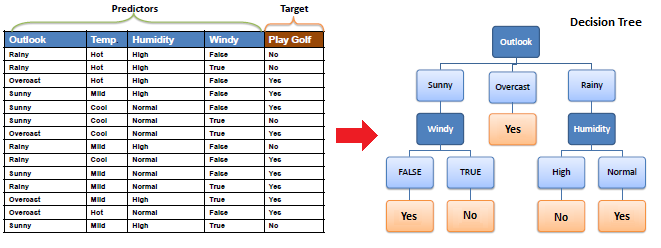
\includegraphics{classification tree.png}

Purpose: Classify data into discrete categories based on certain
features.

Example: Deciding whether to play golf based on weather conditions
(temperature, rainfall, wind).

Classification trees, similar with flowcharts, systematically classify
data into discrete categories based on its features, like deciding to
play golf depending on weather conditions. Starting from the root node,
a split is established by solving an optimization problem (usually
minimizing an impurity measure), before proceeding to recurse on the two
resulting child nodes (Bertsimas and Dunn 2017). Each node in the tree
makes a decision, categorizing the data into different paths based on
specific criteria or thresholds. The decision to split at each node is
often based on criteria such as Gini impurity, the goal is to choose
splits that decrease Gini impurity, leading to a more accurate
classification.

\subsection{Regression Trees}\label{regression-trees}

Purpose: Predict a continuous dependent variable. Example: Predicting
GCSE scores, where linear regression is inadequate due to non-linear
relationships and large residuals. Data is divided into smaller subsets
using decision trees, allowing for more precise predictions in cases
where a simple linear model fails. The decision to split data is based
on reducing the sum of squared residuals (SSR), aiming for the lowest
SSR at each split. The initial split (root of the tree) is chosen based
on the threshold that minimizes SSR, and this process is repeated for
subsequent splits. To avoid overfitting, a minimum number of
observations can be required before further splitting.

\subsection{overfitting:}\label{overfitting}

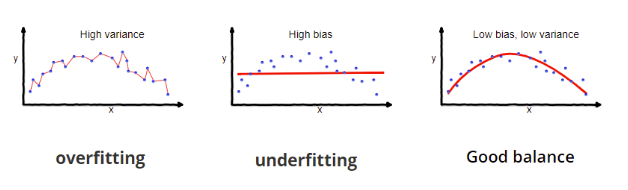
\includegraphics{overfitting.png}

Overfitting, with high variance and low bias occurs when a model learns
the training data too well. his happens often with very complex models
that have too many parameters relative to the number of observations.
While such a model may perform exceptionally well on the training data,
its performance usually drops significantly on new, unseen data because
it has essentially memorized the training data rather than learning the
general underlying patterns. Weakest link pruning is needed when dealing
with fully grown decision trees that may have overfitted the training
data

Underfitting, with high bias and low variance, occurs when a model is
too simple to capture the underlying structure of the data. This can
happen if the model does not have enough parameters (or complexity) to
learn from the data

Thus we are aiming for good balance with low bias and low variance,
performs well on the training data and maintains good performance on
new, unseen data.

\subsection{Random Forests}\label{random-forests}

Fig from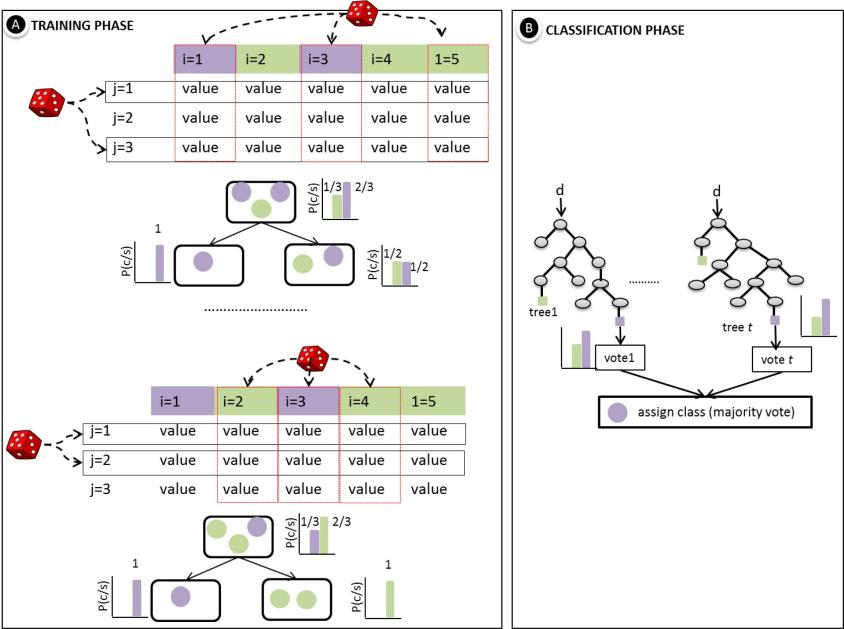
\includegraphics{RF.png}

A random forest (RF) classifier is an ensemble classifier that uses a
randomly chosen subset of training samples and variables to generate
several decision trees ((Belgiu and Drăguţ 2016)). In contrast to
alternative approaches, the RFR model can handle large data
dimensionality and multicollinearity and is less sensitive to noise and
overfitting (Wang et al. 2016)

It enhance decision tree performance by aggregating predictions from
multiple trees, reducing overfitting and improving accuracy: Uses random
samples with replacement to create diverse trees. At each split, selects
a random subset of features, increasing tree diversity. Repeats sampling
and feature selection to create many trees, forming a forest. Each tree
votes on predictions; the majority vote decides the final prediction.
Estimates prediction error using data not sampled for each tree,
providing an unbiased error estimate. Trees grow to their full size
without pruning, relying on the ensemble to prevent overfitting.
Typically, the number of features considered at each split is the square
root of the total number of features.

\subsection{Unsupervised
classification}\label{unsupervised-classification}

Unsupervised classification, often called clustering, includes
techniques like k-means and DBSCAN, which categorize data based on
features like spectral space and distance metrics

\subsection{Supervised classification}\label{supervised-classification}

Supervised classification is a method used to categorize data into
predefined groups or classes based on training data that is already
labeled.

\subsection{Support Vector Machine
(SVM)}\label{support-vector-machine-svm}

is a powerful tool in machine learning for sorting data into categories.
Here's a simpler breakdown of what it does:

draw a line (or a plane in higher dimensions when there are more then 2
datasets) that best separates different types of data points.

SVM looks for the line that keeps the maximum distance from the closest
points of any category, ensuring it's not just separating but also
maximizing the space between these categories. These closest points are
called support vectors.

Two main settings, C and Gamma, help adjust how strict the model is. A
higher C makes the boundary stricter but might only focus on the most
challenging points to separate. Gamma affects how much influence each
data point has; a high Gamma means only nearby points matter much.

Sometimes data isn't easily separable with a straight line. SVM can
twist and turn the data (using something called the kernel trick) to
find a way to separate it effectively.

\bookmarksetup{startatroot}

\chapter{Application}\label{application-3}

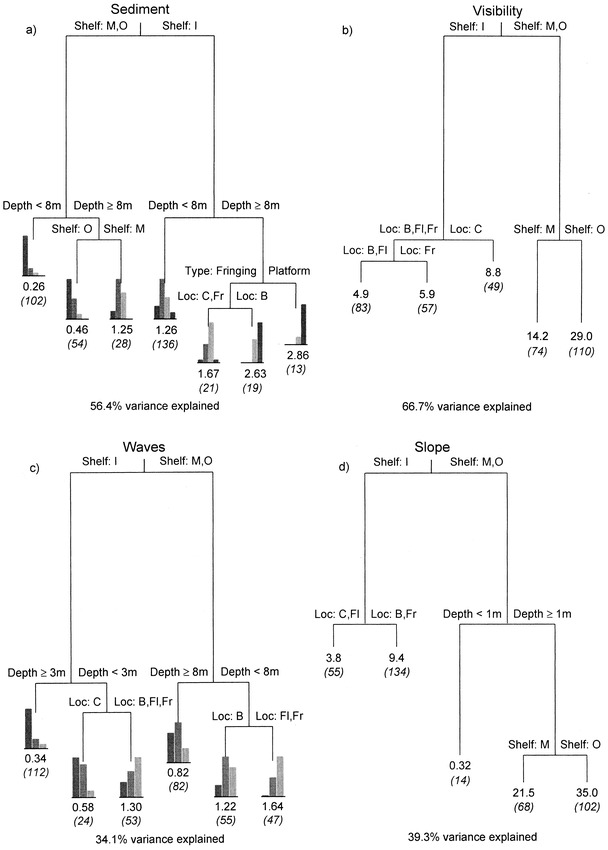
\includegraphics{CART.png}

Fig from (De'ath and Fabricius 2000)

Classification and regression trees are ideally suited for the analysis
of complex ecological data. In this study (De'ath and Fabricius 2000) we
evaluate survey data, including physical and spatial environmental
variables and abundances of soft coral species (Cnidaria: Octocorallia)
from the Australian central Great Barrier Reef using regression trees
and categorization. Dense aggregations, usually consisting of three
taxa, were found to be limited to specific habitat categories, each of
which was determined by a combination of three to four environmental
variables, according to regression tree analyses. The study found that
both physical and spatial variables were effective predictors of soft
coral abundances, and spatial variables could act as surrogates for
physical variables in extensive reef complexes where physical data might
be unavailable. The case study also illustrated the advantage of CART
over linear models in uncovering patterns in the data\hspace{0pt}

Regression trees connecting the four spatial variables (shelf position,
location, reef type, and depth) to the distributions of the four
physical variables (sediment, visibility, waves, and slope).

In the case study conducted in Bangladesh (Zhao et al. 2019), the Random
Forest Regression (RFR) model was used to estimate poverty using data
from multiple sources, including nighttime light data, Google satellite
imagery, land cover map, road map, and division headquarter location
data. The household wealth index (WI) from the Demographic and Health
Surveys (DHS) was the measure of poverty. The RFR model's effectiveness
stems from its ability to handle various data types, manage high
dimensionality, and cope with multicollinearity, leading to a more
accurate and reliable poverty estimation compared to traditional
methods.

Here is the dataset used in this study.

\includegraphics[width=6.8125in,height=\textheight]{RFR.png}

Fig from (Zhao et al. 2019)

\begin{enumerate}
\def\labelenumi{(\alph{enumi})}
\tightlist
\item
  Wealth Index (WI) map, (b) National Polar-orbiting Partnership Visible
  Infrared Imaging Radiometer Suite (NPP-VIIRS) nighttime light (NTL)
  image, (c) Open Street Map (OSM) primary and secondary road map, (d)
  land cover map
\end{enumerate}

The model demonstrated good predictive power and generalization ability.
The use of The methodology was efficient in measuring poverty due to
RFR's robust handling of complex and varied data

The two articles showcase the application of machine learning
techniques, specifically Classification and Regression Trees (CART) and
Random Forest Regression (RFR), in both ecological and socioeconomic
analyses. These studies demonstrate the flexibility and utility of these
methods in addressing complex, multidimensional issues across different
fields.

RFR, an ensemble method that combines multiple decision trees, has shown
improved accuracy and robustness compared to single decision trees. RFR
is crucial in poverty measurement, as poverty is multifaceted,
influenced by various socioeconomic and environmental factors, thus it,
together with many similar social-related issues, should be measured by
multi-source datasets. Also RFR can handle multicollinearity better then
CART, as in social sciences, many variables can be interrelated, which
complicates the analysis. So for complex issues like poverty
measurement, where accuracy, the handling of multicollinear data, and
robustness to noise are required, RFR is usually a suitable method.

\bookmarksetup{startatroot}

\chapter{Reflection}\label{reflection-3}

This week's exploration of classifying remotely sensed data using
machine learning is similar with human inference. What I found useful in
the further study is classification trees and regression trees, with
applications ranging from weather-based activities to predicting
educational outcomes. The concept of overfitting and underfitting
brought me back to the memory of learning regression models.

Random Forests (RF) gave me an idea of how to avoid the bad effects of
multicollinearity similar with the knowledge from multi-linear
regression. It can handle large datasets and complex interactions
through gathering decision trees, reducing overfitting and enhancing
predictive accuracy. This was practically useful in studies like coral
species analysis and poverty estimation.

Unsupervised methods like k-means and supervised techniques, including
Support Vector Machines (SVM), expanded my understanding of machine
learning's diversity.\\
Through these insights, I gained a holistic view of machine learning's
role in data analysis, from theoretical foundations to real-world
applications.

\section{\texorpdfstring{\textbf{Reference}}{Reference}}\label{reference}

\bookmarksetup{startatroot}

\chapter{week\_8}\label{week_8}

\bookmarksetup{startatroot}

\chapter{Summary}\label{summary-2}

\section{Object-Based Image Analysis
(OBIA)}\label{object-based-image-analysis-obia}

OBIA shifts focus from individual pixels to shapes or superpixels,
based on their homogeneity (similarity) or heterogeneity (difference).
SLIC (Simple Linear Iterative Clustering) is a common method for
generating superpixels, analyzing spatial and color distances to define
groups. Iterative process, typically 4-10 rounds, refines superpixel
centers and boundaries, similar to k-means. Uses LAB color space for
nuanced color analysis, classifying objects based on average values for
interpretation.

The basic logic is: Divide the image into items that correspond to
land-based features, and then categorize them based on their dimensions,
spectral characteristics, form, and size (Geography 2024).

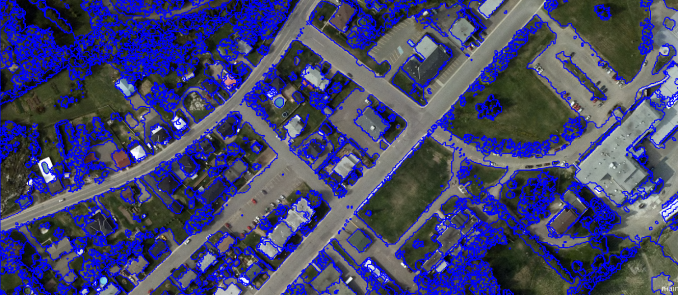
\includegraphics{OBIA1.png}

Object-Based Image Analysis (OBIA) segmentation is a process that groups
similar pixels into objects (Geography 2024).

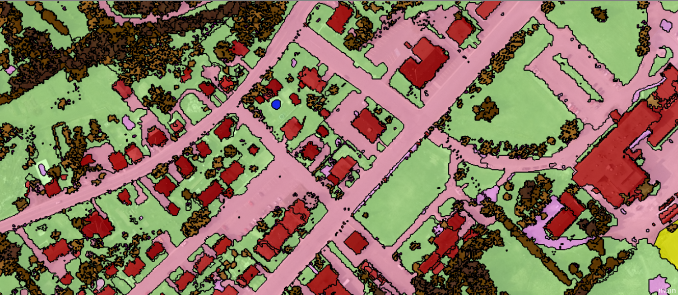
\includegraphics{OBIA2.png}

OBIA classification uses shape, size, and spectral properties of objects
to classify each object (Geography 2024).

\section{Sub pixel analysis}\label{sub-pixel-analysis}

Allows us to deconstruct the observed spectral data of a pixel into its
constituent materials, giving us a clearer understanding of what is
present on the ground in that area.

End Members: In the context of remote sensing, ``end members'' are pure
spectral signatures representing specific materials or objects on the
ground, such as water, vegetation, and soil.

Pixel Modeling: The goal here is to determine what mixture of these end
members (water, vegetation, soil) makes up a single pixel in an image

Calculkation method: The left side of the equation represents the
spectral signature of a pixel in bands 3 and 4, plus the condition that
the sum of the fractions of end members equals 1. The matrix in the
middle represents the spectral signatures of the end members (water,
vegetation, soil) for bands 3 and 4, with an additional row of ones to
enforce the sum-to-one constraint. The right side represents the
fractions of each end member within the pixel that we are trying to
find. Then calculate fraction by forming a new matrix with the left hand
side being the fraction matrix, and the calculated value is the
proportion of the different end members.

\section{Accuracy assessment}\label{accuracy-assessment}

in machine learning is a process to evaluate how well a model's
predictions match the actual reality

True Positive (TP): The model correctly predicts the positive class.

False Positive (FP): The model incorrectly predicts the positive class.

True Negative (TN): The model correctly predicts the negative class.

False Negative (FN): The model incorrectly predicts the negative class.

Accuracy assessment is can be divided into producer's accuracy
((TP)/(TP+FN), user's accuracy (TP)/(TP+FP), and overall
accuracy~(TP)+(TN)/(TP+TN+FP+FN).

Sometimes producer's accuracy is high as for example, 21 out of 22 urban
areas were being recognized, however a user may find that only 22/31 of
the time visit an urban area is it actually urban. 1.4 Receiver
Operating Characteristic Curve Developed during WW2 by the USA to
enhance radar signal detection, aiming to identify aircraft (true
positives) while minimizing false alarms (false positives) from other
objects like clouds.

Threshold Adjustment: Altering the classifier's threshold affects the
TPR and FPR, allowing for the optimization of the classifier's
performance based on the ROC curve.

The aim is to maximize true positives (aiming for a TPR of 1) while
minimizing false positives (aiming for an FPR of 0), optimizing the
classifier's accuracy

A perfect model scores 1, while a random guess scores 0.5, the higher
the AUC, the better the model is at predicting true positives

\section{Cross validation and spatial
autocorrelation.}\label{cross-validation-and-spatial-autocorrelation.}

When we're working with data in geography or maps, we usually divide our
data into two parts: one part to learn from (train) and another part to
see how well we've learned (test). However, there's an important idea by
Waldo Tobler, called the ``First Law of Geography,'' which says that
things that are closer to each other are more alike than things that are
far apart. This means when we're training our model, if the training
data includes information that's very close to the test data, it might
provide `sneak peek' because the training data shouldn't know anything
about the test data.

In this figure, we prefer the lower row as the upper one's training data
and test data are near each other.

\section{SVM (Support Vector Machine
classifier)}\label{svm-support-vector-machine-classifier}

SVMs are a group of supervised learning techniques used in regression
analysis, outlier identification, and classification ({``Support Vector
Machines in Scikit-Learn''} 2023).~

C (Penalty parameter): Controls the strictness of the SVM; lower C
allows more misclassifications, higher C aims for precise
classification.

Gamma (σ): Affects the influence of data points; lower Gamma leads to
broader grouping, higher Gamma results in tighter, smaller groups.

To optimize C and Gamma, they employ spatial fold division, using
k-means to separate data into distinct spatial folds, ensuring unbiased
training and testing.

They conduct cross-validation within these folds, with each spatial
partition undergoing 5-fold validation, assessing 50 random
hyperparameter sets, resulting in 1,250 models per cycle.

Repeating the process 100 times, they evaluate 125,000 models to
determine the ideal SVM settings.

\bookmarksetup{startatroot}

\chapter{Application:}\label{application-4}

In the case study VerbeirenEtAl2008 (Verbeiren et al. 2008), sub-pixel
classification was used to estimate regional crop areas in Belgium using
low-resolution SPOT-VEGETATION NDVI images. It proved effective for
generating reliable area estimates in regions with limited
high-resolution data.

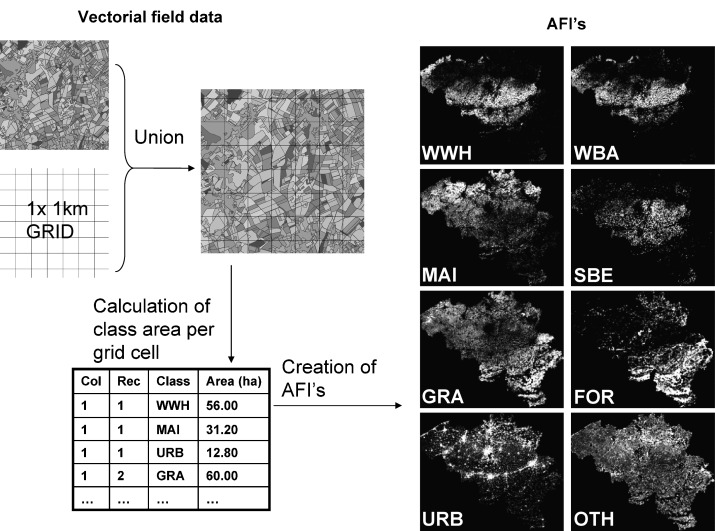
\includegraphics{sub-pixel.png}

Figure from (Verbeiren et al. 2008)

These AFIs (area fraction images) have the same 1~km resolution as the
satellite images and they give for each pixel the area fraction occupied
by the considered classes (per pixel, the fractions sum up to 1). The
procedure for the AFI-creation is outlined in~the picture. First, a
1~km~×~1~km grid was created with the same spatial characteristics
(projection, resolution, framing) as the NDVI-images. This grid was
superimposed over the vectorial land use map, and the area fractions of
the eight classes (Winter wheat, Winter barley, All maize, Sugar beets,
All grassland, All forests, Urban areas, and All other vegetation)
within each grid cell were computed and stored in a database. The latter
numbers were then transferred to eight separate images: the (reference)
AFIs.

Literature 2

Object - based image analysis is also very useful. Building damage
detection after earthquake would help to rapid relief and response of
disaster. In this study (Janalipour and Mohammadzadeh 2016), an
efficient method was proposed for building damage detection in urban
area after earthquake using pre-event vector map and postevent
pan-sharpened high spatial resolution image. At first, preprocessing was
applied on the postevent satellite image. Second, results of pixel- and
object-based classifications were integrated. In the following,
geometric features of buildings were extracted including area,
rectangular fit (rect\_fit), and convexity.~

After a series of image analysis, we are able to define the category of
the land as well as the degree of damage.

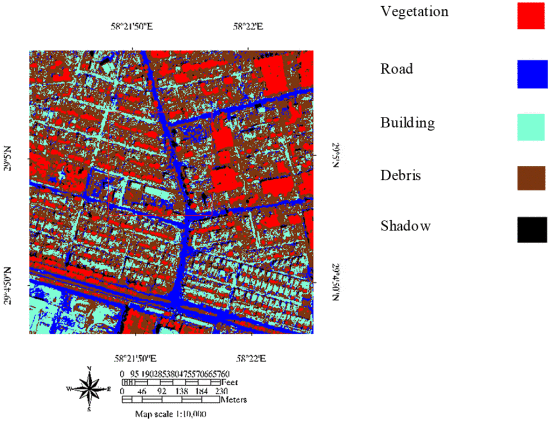
\includegraphics[width=3.29167in,height=\textheight]{OBIA.png}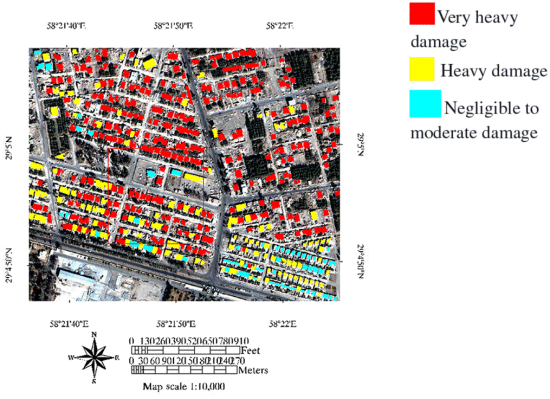
\includegraphics[width=3.29167in,height=\textheight]{OBIA_b.png}

Figures from (Janalipour and Mohammadzadeh 2016)

\bookmarksetup{startatroot}

\chapter{Reflection}\label{reflection-4}

Reflecting on my learning journey through the class, I've learned many
image analysis techniques, notably Object-Based Image Analysis (OBIA)
and sub-pixel analysis. The OBIA method, groups pixels into objects
based on their spectral, spatial, and textural characteristics, I found
it particularly useful in areas like land use classification. Sub-pixel
analysis helped me understand image analysis further by breaking down
the spectral signatures within a pixel, thereby providing a clearer
picture of the ground realities.

It was enlightening to see how famous concepts like the First Law of
Geography play an important role in practical sections like
cross-validation, impacting models' reliability.

The application in assessing building damage after earthquake
demonstrated the key use of OBIA, showing how these technologies can
significantly contribute to disaster response and management.

Overall, this class deepened my knowledge of the image analysis
techniques and their practical implications in environmental monitoring
and disaster management.

\bookmarksetup{startatroot}

\chapter*{References}\label{references-1}
\addcontentsline{toc}{chapter}{References}

\markboth{References}{References}

\phantomsection\label{refs}
\begin{CSLReferences}{1}{0}
\bibitem[\citeproctext]{ref-BelgiuDragut2016}
Belgiu, M., and L. Drăguţ. 2016. {``Random Forest in Remote Sensing: A
Review of Applications and Future Directions.''} \emph{ISPRS Journal of
Photogrammetry and Remote Sensing} 114: 24--31.

\bibitem[\citeproctext]{ref-BertsimasDunn2017}
Bertsimas, D., and J. Dunn. 2017. {``Optimal Classification Trees.''}
\emph{Machine Learning} 106 (7): 1039--82.

\bibitem[\citeproctext]{ref-DeathFabricius2000}
De'ath, Glenn, and K. E. Fabricius. 2000. {``Classification and
Regression Trees: A Powerful yet Simple Technique for Ecological Data
Analysis.''} \emph{Ecology} 81 (11): 3178--92.

\bibitem[\citeproctext]{ref-GISGeographyOBIA2024}
Geography, GIS. 2024. {``OBIA - Object-Based Image Analysis (GEOBIA).''}
\url{https://gisgeography.com/obia-object-based-image-analysis-geobia/}.

\bibitem[\citeproctext]{ref-JanalipourMohammadzadeh2016}
Janalipour, M., and A. Mohammadzadeh. 2016. {``Building Damage Detection
Using Object-Based Image Analysis and ANFIS from High-Resolution Image
(Case Study: BAM Earthquake, Iran).''} \emph{IEEE Journal of Selected
Topics in Applied Earth Observations and Remote Sensing} 9 (5):
1937--45.

\bibitem[\citeproctext]{ref-knuth84}
Knuth, Donald E. 1984. {``Literate Programming.''} \emph{Comput. J.} 27
(2): 97--111. \url{https://doi.org/10.1093/comjnl/27.2.97}.

\bibitem[\citeproctext]{ref-ScikitLearnSVM}
{``Support Vector Machines in Scikit-Learn.''} 2023.
\url{https://scikit-learn.org/stable/modules/svm.html}.

\bibitem[\citeproctext]{ref-VerbeirenEtAl2008}
Verbeiren, S. et al. 2008. {``Sub-Pixel Classification of
SPOT-VEGETATION Time Series for the Assessment of Regional Crop Areas in
Belgium.''} \emph{International Journal of Applied Earth Observation and
Geoinformation} 10 (4): 486--97.

\bibitem[\citeproctext]{ref-WangEtAl2016}
Wang, L. a., X. Zhou, X. Zhu, Z. Dong, and W. Guo. 2016. {``Estimation
of Biomass in Wheat Using Random Forest Regression Algorithm and Remote
Sensing Data.''} \emph{The Crop Journal} 4: 212--19.

\bibitem[\citeproctext]{ref-ZhaoEtAl2019}
Zhao, X. et al. 2019. {``Estimation of Poverty Using Random Forest
Regression with Multi-Source Data: A Case Study in Bangladesh.''}
\emph{Remote Sensing} 11 (4): 375.

\end{CSLReferences}



\end{document}
